\documentclass{article}
\usepackage[utf8]{inputenc}
\usepackage{graphicx}
\usepackage{amsfonts}       % blackboard math symbols

\setlength{\parindent}{1cm} % espaçamento do parágrafo
\usepackage{geometry} % configurar layout da página
\usepackage{setspace} % configurar o espaçamento de linhas
\usepackage{indentfirst} % alinhamento do texto, parágrafos

\graphicspath{ {./images/} }

\usepackage{float} % tabela que nao fica fixa

\usepackage{siunitx}  % Package perfeita pra notacao cientifica
\RequirePackage{amsmath,amsthm,amssymb,hyperref} % Math 

\title{ENGC46 - Síntese de Circuitos: Trabalho I}
\date{Semestre Letivo Suplementar 2020 - Universidade Federal da Bahia}
\author{Henrique Nunes Poleselo}

\begin{document}

\maketitle

\section{Especificações}
O objetivo é projetar um filtro RC ativo com a seletividade rejeita-faixa com as seguintes especificações:
\begin{itemize} 
    \item Banda de Passagem: 500Hz - 20MHz
    \item Banda de Rejeição: 35kHz - 80kHz
    \item Amax: 0.2dB
    \item Amin: 40dB
    \item Função de Aproximação: Butterworth
    \item Arquitetura: K-H-N (Kerwin-Huelsman-Newcomb)
\end{itemize}


\section{Projeto}

Um filtro rejeita faixa é caracterizado pela seguinte função de transferência:

\begin{equation}
    T(s) = Kmax \cdot \frac{ s^2 + wo^2 }{s^2 + \frac{wo}{Q} s + wo^2}.
\end{equation}

Onde o termo de primeira ordem do númerador é 0. Dada as especificações, para a realização do filtro, usou-se a aproximação de Butterworth. Para a obtenção da aproximação utilizou-se o MATLAB. O código fonte encontra-se em anexo juntamente com este relatório. Para melhor ilustração, os \textit{snippets} do código em questão:

\begin{center}
\centering
  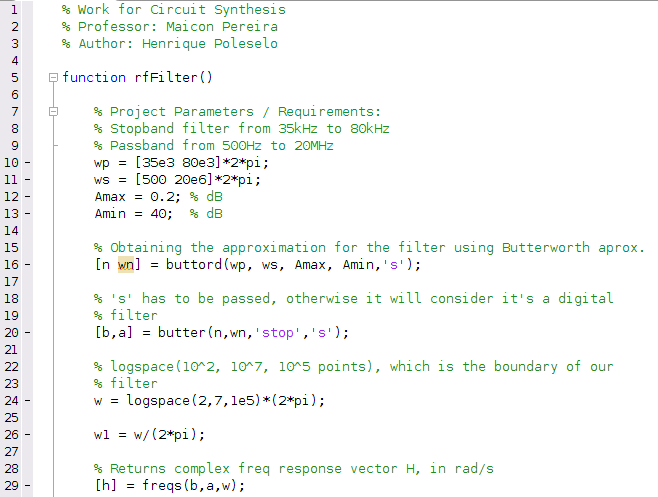
\includegraphics[scale=0.8]{img/code1.png}
\end{center}

\begin{center}
\centering
  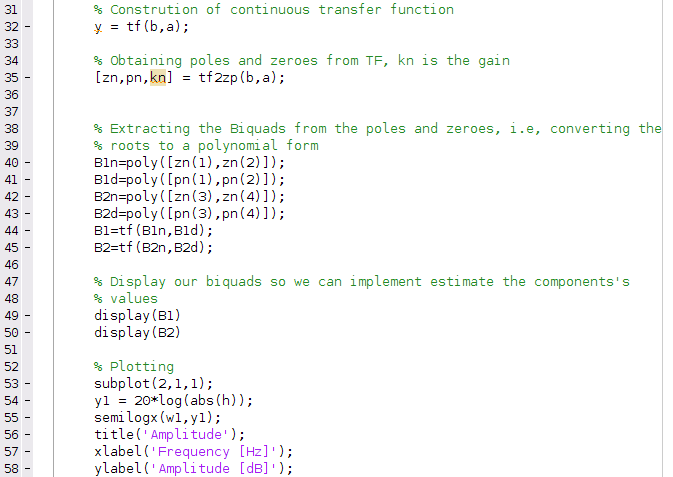
\includegraphics[scale=0.8]{img/code2.png}
\end{center}

\begin{center}
\centering
  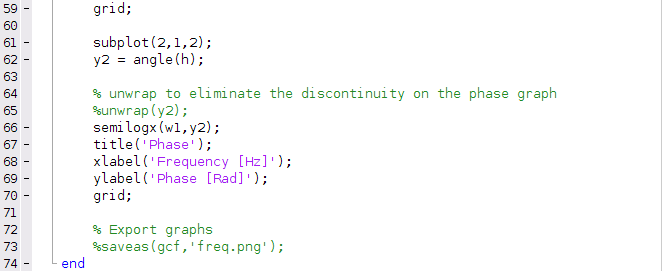
\includegraphics[scale=0.8]{img/code3.png}
\end{center}


Os biquads obtidos foram:
\begin{center}
\centering
  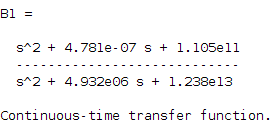
\includegraphics[scale=0.8]{img/biquad1.png}
\end{center}

\begin{center}
\centering
  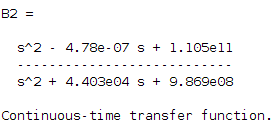
\includegraphics[scale=0.8]{img/biquad2.png}
\end{center}

Como um dos requisitos é a arquitetura biquad $KHN$, seguindo a estrutura de múltiplos amplificadores operacionais de forma a ter mais estabilidade, usou-se o seguinte circuito generalizado para a implementação do filtro:

\begin{center}
\centering
  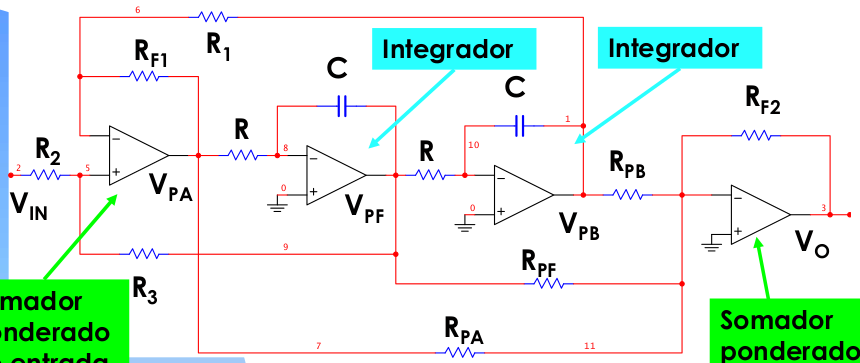
\includegraphics[scale=0.5]{img/circuitokhn.png}
\end{center}

\begin{center}
\centering
  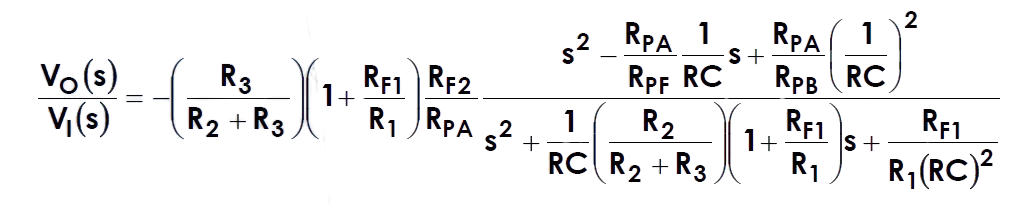
\includegraphics[scale=0.5]{img/modelogeral.png}
\end{center}

Igualou-se os valores que multiplicam os termos em $s$ dos respectivos biquads encontrados com as expressões que multiplicam os termos em $s$ da forma geral de $KHN$, de forma a dimensionar-se o valor dos componentes.

Para um filtro rejeita-faixa o termo de primeiro grau $s$ do númerador precisa ser 0, portanto uma condição para os dois biquads encontrados é:

\begin{equation}
    \frac{RPA}{RPF \cdot R \cdot C} = 0
\end{equation}

Além disso, o termo de grau 0 em $s$ dos dois biquads foi igual, portanto uma condição igualitária para ambos:

\begin{equation}
    \frac{RPA}{RPB \cdot R^2 \cdot C^2} = \num{1.105e11}
\end{equation}


Para o primeiro biquad:

\begin{equation}
    \frac{RF1}{R1 \cdot R^2 \cdot C^2} = \num{1.238e13}
\end{equation}

e

\begin{equation}
    \frac{1}{R \cdot C} \frac{R2}{R2+R3} \cdot (1+ \frac{RF1}{R1} )= \num{4.932e6}
\end{equation}

O mesmo procedimento foi feito para o segundo biquad:

\begin{equation}
    \frac{RF1}{R1 \cdot R^2 \cdot C^2} = \num{9.869e8}
\end{equation}

e

\begin{equation}
    \frac{1}{R \cdot C} \frac{R2}{R2+R3} \cdot (1+ \frac{RF1}{R1} )= \num{4.403e4}
\end{equation}


Uma tabela em formato excel foi feita de forma a auxiliar o dimensionamento dos resistores. A mesma se encontra em anexo juntamente com este relatório. Os valores encontrados para os resistores foram:

\begin{table}[H]
\centering
\begin{tabular}{|c|c|c|c|l}
\cline{1-4}
 R & 100 & RF2 & 0.0073888  \\ \cline{1-4}
 R1 & \num{1e5} & RPB & 90.09  \\ \cline{1-4}
 R2 & 100 & RPF & \num{1.5e10}  \\ \cline{1-4}
 R3 & \num{3.68e15} & RPA & 10  \\ \cline{1-4}
 RF1 & \num{1.24e6} & C & \num{10e-9}  \\ \cline{1-4}
\end{tabular}
\caption{valores do Biquad 1: resistores dados em \si{\ohm} e Capacitor em farads $F$ calculados pela planilha}
\end{table}

\begin{table}[H]
\centering
\begin{tabular}{|c|c|c|c|l}
\cline{1-4}
 R & 100 & RF2 & 0.99  \\ \cline{1-4}
 R1 & \num{1e5} & RPB & 900.9  \\ \cline{1-4}
 R2 & 100 & RPF & \num{1.61e11}  \\ \cline{1-4}
 R3 & \num{4.4e14} & RPA & 100  \\ \cline{1-4}
 RF1 & 98.7 & C & \num{10e-9}  \\ \cline{1-4}
\end{tabular}
\caption{valores do Biquad 2: resistores dados em \si{\ohm} e Capacitor em farads $F$ calculados pela planilha}
\end{table}

Com os valores dimensionados, partiu-se para a simulação no $LTSpice$:

\begin{center}
\centering
  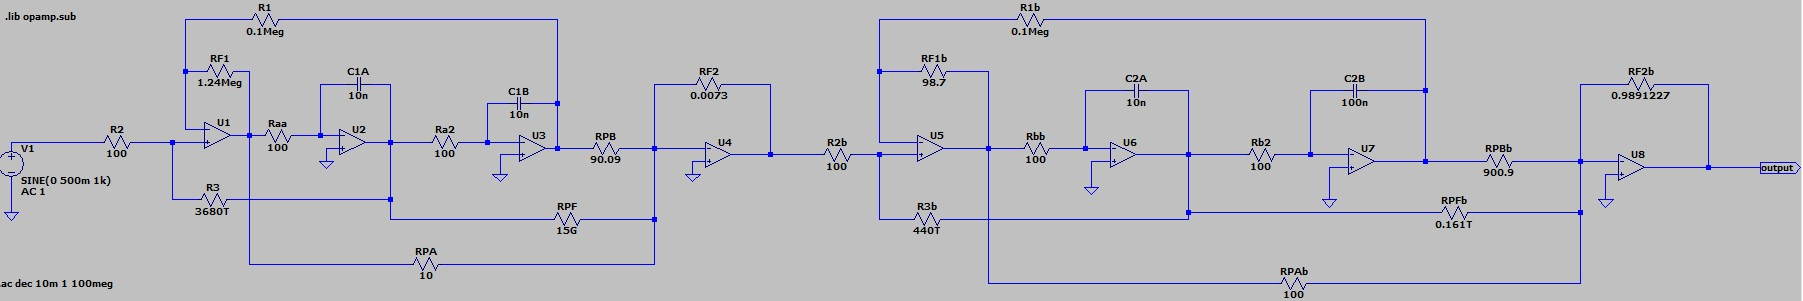
\includegraphics[scale=0.35]{img/CircuitoMontado.jpg}
\end{center}

Uma comparação da magnitude da resposta em frequência do circuito simuldo através do $LTSpice$ e da aproximação feita no MATLAB: 

\begin{center}
\centering
  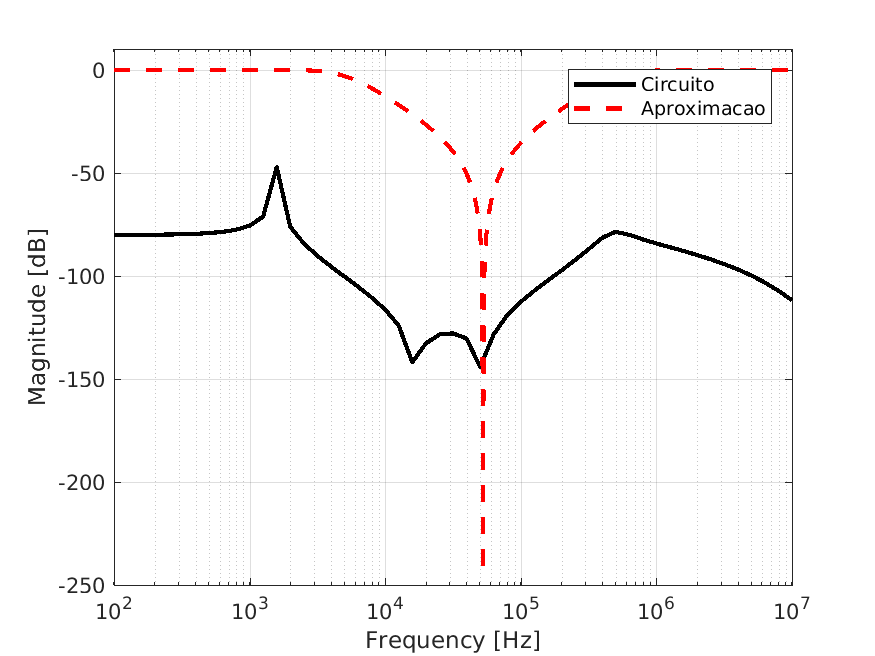
\includegraphics[scale=0.8]{img/result.png}
\end{center}



O mesmo para a fase:

\begin{center}
\centering
  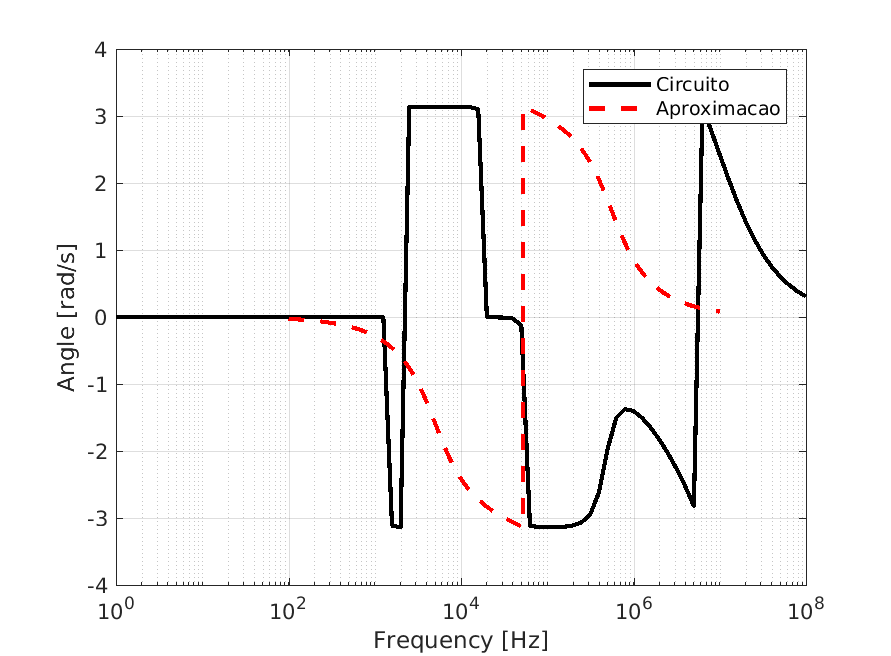
\includegraphics[scale=0.8]{img/phase.png}
\end{center}


\end{document}